%%%%%%%%%%%%%%%%%%%%%%%%%%%%%%%%%%%%%%%%%%%%%%%%%%%%%%%%%%%%%%%%%%%%%%%%%%%%%%%%
%%%%%%%%%%%%%%%%%%%%%%%%%%%%%%%%%%%%%%%%%%%%%%%%%%%%%%%%%%%%%%%%%%%%%%%%%%%%%%%%
%
% A general frame for lecture slides and lecture notes in one file
% using LaTeX beamer
%
%%%%%%%%%%%%%%%%%%%%%%%%%%%%%%%%%%%%%%%%%%%%%%%%%%%%%%%%%%%%%%%%%%%%%%%%%%%%%%%%
%%%%%%%%%%%%%%%%%%%%%%%%%%%%%%%%%%%%%%%%%%%%%%%%%%%%%%%%%%%%%%%%%%%%%%%%%%%%%%%%

% only for the article version
\mode<article> 
{
  \usepackage[automark,komastyle]{scrpage2}
  \usepackage{amsfonts}
  \usepackage{amsthm}
  \usepackage{amscd}
  \usepackage{fullpage}
  \setlength{\parindent}{0pt}
  \setlength{\parskip}{1.3ex plus 0.5ex minus 0.2ex}
}

% only presentation 
\mode<presentation>
{
%  \usepackage{times}
%  \usetheme{default}
  \usetheme[secheader]{Boadilla}
  \setbeamercovered{transparent}
  \setbeamertemplate{background canvas}[vertical shading][bottom=white!10,top=white!10]
  \setlength{\parindent}{0pt}
  \setlength{\parskip}{1.35ex plus 0.5ex minus 0.3ex}
  \setbeamertemplate{theorems}[numbered]
  \usefonttheme[onlysmall]{structurebold}
  \usepackage{amscd}
}

% all after
\usepackage{graphicx}
%\usepackage{multimedia}
\usepackage{psfrag}
\usepackage{listings}
\lstset{language=C++, basicstyle=\ttfamily,
  stringstyle=\ttfamily, commentstyle=\it, extendedchars=true}
\usepackage{curves}
%\usepackage{epic}
\usepackage{calc}
\usepackage{picinpar}
%\usepackage{fancybox}
%\usepackage{xspace}
\usepackage{enumerate}
\usepackage{algorithmic}
\usepackage{algorithm}

\mode<article> 
{
\usepackage{hyperref}
}

%The theorems
\mode<article> 
{
\newtheoremstyle{mystyle}%
{3pt}%
{3pt}%
{}%
{}%
{\sffamily\bfseries}%
{.}%
{.5em}%
{}%
\theoremstyle{mystyle}
}
\mode<presentation> 
{
\theoremstyle{definition}
}
\newtheorem{Def}{Definition}%[section]
\newtheorem{Exm}[Def]{Example}
\newtheorem{Lem}[Def]{Lemma}
\newtheorem{Rem}[Def]{Remark}
\newtheorem{Rul}[Def]{Rule}
\newtheorem{Thm}[Def]{Theorem}
\newtheorem{Cor}[Def]{Corollary}
\newtheorem{Obs}[Def]{Observation}
\newtheorem{Ass}[Def]{Assumption}
\newtheorem{Pro}[Def]{Property}
\newtheorem{Alg}[Def]{Algorithm}
\newtheorem{Prp}[Def]{Proposition}

% Delete this, if you do not want the table of contents to pop up at
% the beginning of each subsection:
\AtBeginSection[]
{
  \begin{frame}<beamer>
    \frametitle{Contents}
\tableofcontents[currentsection,sectionstyle=show/hide,subsectionstyle=show/show/hide]
%    \tableofcontents[currentsection]
  \end{frame}
}

% Title definition
\mode<presentation>
{
  \title{\texttt{dune-pdelab} Howto}
  \author{Peter Bastian}
  \institute[IWR]
  {
    Universit�t Heidelberg\\
    Interdisziplin�res Zentrum f�r Wissenschaftliches Rechnen\\
    Im Neuenheimer Feld 368, D-69120 Heidelberg\\
	email: \url{Peter.Bastian@iwr.uni-stuttgart.de}
  }
  \date{\today}
  \logo{
\includegraphics[width=9mm]{./EPS/iwrlogo-klein.eps}}
}
\mode<article>
{
  \title{\texttt{dune-pdelab} Howto}
  \author{\textsc{Peter Bastian}\\
    Universit�t Heidelberg\\
    Interdisziplin�res Zentrum f�r Wissenschaftliches Rechnen\\
    Im Neuenheimer Feld 368, D-69120 Heidelberg\\
	email: \url{Peter.Bastian@iwr.uni-stuttgart.de}
  }
  \date{\today}
}

% logo nach oben
\mode<presentation>
{
% No navigation symbols and no lower logo
\setbeamertemplate{sidebar right}{}

% logo
\newsavebox{\logobox}
\sbox{\logobox}{%
    \hskip\paperwidth%
    \rlap{%
      % putting the logo should not change the vertical possition
      \vbox to 0pt{%
        \vskip-\paperheight%
        \vskip0.35cm%
        \llap{\insertlogo\hskip0.1cm}%
        % avoid overfull \vbox messages
        \vss%
      }%
    }%
}

\addtobeamertemplate{footline}{}{%
    \usebox{\logobox}%
}
}

% number equations within sections in article mode
%\numberwithin{equation}{section}

% math symbols
\newcommand{\diffd}{\,d}

%%%%%%%%%%%%%%%%%%%%%%%%%%%%%%%%%%%%%%%%%%%%%%%%%%%%%%%%%%%%%%%%%%%%%%%%%%%%%%%%
%%%%%%%%%%%%%%%%%%%%%%%%%%%%%%%%%%%%%%%%%%%%%%%%%%%%%%%%%%%%%%%%%%%%%%%%%%%%%%%%
%
% now comes the individual stuff lecture by lecture
%
%%%%%%%%%%%%%%%%%%%%%%%%%%%%%%%%%%%%%%%%%%%%%%%%%%%%%%%%%%%%%%%%%%%%%%%%%%%%%%%%
%%%%%%%%%%%%%%%%%%%%%%%%%%%%%%%%%%%%%%%%%%%%%%%%%%%%%%%%%%%%%%%%%%%%%%%%%%%%%%%%
\mode<article>
{
\pagestyle{scrheadings}
}

\begin{document}

\mode<presentation>
{
  \begin{frame}
    \titlepage
  \end{frame}
}
\mode<article>
{
\maketitle
}

\begin{abstract}
This article contains concepts for a general discretization module for
the ``Distributed Numerics Environment'' (DUNE). It should enable one
to build up a library of finite element methods in an easy and
extendable way that is closely related to the mathematical formulation
of finite element method. As the first necessary step an abstract
framework for formulating a large variety of finite element methods is
attempted. 
\end{abstract}

\mode<article>
{
\cleardoublepage
}

\mode<presentation>{
\begin{frame}<presentation>
\frametitle{Outline}
\tableofcontents[section,sectionstyle=show/show,subsectionstyle=hide/hide/hide] 
\end{frame}
}

\mode<article>
{
\tableofcontents
}

\mode<article>
{
\cleardoublepage
}

%%%%%%%%%%%%%%%%%%%%%%%%%%%%%%%%%%%%%%%%%%%%%%%%%%%%%%%%%%%%
%%%%%%%%%%%%%%%%%%%%%%%%%%%%%%%%%%%%%%%%%%%%%%%%%%%%%%%%%%%%
%%%%%%%%%%%%%%%%%%%%%%%%%%%%%%%%%%%%%%%%%%%%%%%%%%%%%%%%%%%%
\section{Introduction}
%%%%%%%%%%%%%%%%%%%%%%%%%%%%%%%%%%%%%%%%%%%%%%%%%%%%%%%%%%%%
%%%%%%%%%%%%%%%%%%%%%%%%%%%%%%%%%%%%%%%%%%%%%%%%%%%%%%%%%%%%
%%%%%%%%%%%%%%%%%%%%%%%%%%%%%%%%%%%%%%%%%%%%%%%%%%%%%%%%%%%%

\subsection{What is missing in DUNE?}

\cleardoublepage

%%%%%%%%%%%%%%%%%%%%%%%%%%%%%%%%%%%%%%%%%%%%%%%%%%%%%%%%%%%%
%%%%%%%%%%%%%%%%%%%%%%%%%%%%%%%%%%%%%%%%%%%%%%%%%%%%%%%%%%%%
%%%%%%%%%%%%%%%%%%%%%%%%%%%%%%%%%%%%%%%%%%%%%%%%%%%%%%%%%%%%
\section{Weighted Residual Formulation}
%%%%%%%%%%%%%%%%%%%%%%%%%%%%%%%%%%%%%%%%%%%%%%%%%%%%%%%%%%%%
%%%%%%%%%%%%%%%%%%%%%%%%%%%%%%%%%%%%%%%%%%%%%%%%%%%%%%%%%%%%
%%%%%%%%%%%%%%%%%%%%%%%%%%%%%%%%%%%%%%%%%%%%%%%%%%%%%%%%%%%%

\subsection{Abstract Formulation}

When we go about to solve a PDE problem we need a general idea of what
a PDE problem is. We will develop such an idea in this section.

\begin{frame}
\frametitle<presentation>{Weighted Residual Formulation}

\begin{Def}[Weighted Residual Formulation]
We claim that all problems we ever want to solve can be written in the form
\begin{equation}
\text{Find } u_h\in w_h + \tilde{U}_h : \qquad r_h(u_h,v) =
0 \qquad \forall v\in V_h.  
\end{equation}
Where:
\begin{itemize}
\item $\tilde{U}_h\subseteq U_h$, $\tilde{V}_h\subseteq V_h$ are
finite-dimensional function spaces and corresponding subspaces.
\item Affine shift: $u_h\in w_h + \tilde{U}_h$ for a given $w_h\in U_h$ means
$u_h = w_h + \tilde{u}_h$ for some $\tilde{u}_h\in\tilde{U}_h$.
\item $r_h : U_h \times V_h \to \mathbb{K}$ is the \textit{residual form}.
\begin{itemize}
\item $r_h$ may be \textit{nonlinear} in its first argument.
\item $r_h$ \textit{is always linear} in its second argument.
\item $r_h$ may depend on the grid in non-conforming methods.
\end{itemize}
\item We assume that this problem has a unique solution. \hfill$\square$
\end{itemize}
\end{Def}
\end{frame}

We now give some concrete examples.

\subsection{Some Examples}

\paragraph{Continuous Problem}

\begin{frame}
\frametitle<presentation>{Continuous Problem}

Consider the Poisson equation
\begin{subequations}
\label{Eq:DiffusionEquation}
\begin{align}
                -\Delta u &= f& \text{in }& \Omega\subseteq\mathbb{R}^n,\\
                        u &= g& \text{on }& \Gamma_D\subseteq\partial\Omega,\\
     - \nabla u\cdot\nu   &= j& \text{on }& \Gamma_N=\partial\Omega\setminus\Gamma_D,
\end{align}
\end{subequations}
where $\mbox{meas}(\Gamma_D)\neq 0$. 

The \textit{weak formulation} uses the spaces
\begin{equation*}
U = H^1(\Omega), \qquad
\tilde{U} = \{u \in U\,|\, \text{``$u=0$'' on $\Gamma_D$}
\}
\end{equation*}
and reads
\begin{equation}\label{Eq:DiffusionWeakForm}
u \in w+\tilde{U} \  : \quad
\underbrace{\int_\Omega \nabla u \cdot \nabla v \diffd x
+ \int_{\Gamma_N} j v \diffd s - \int_\Omega f v \,dx}_{= r(u,v)} = 0,  
\quad \forall v\in \tilde{U}.
\end{equation}
Here $w\in U$ is a function with ``$w=g$'' on $\Gamma_D$ and $V=U$, $\tilde{V}=\tilde{U}$.
\end{frame}


\paragraph{Conforming Finite Elements of Order $k$}

First we need to introduce some notation for the grid:

\begin{frame}
\frametitle<presentation>{Conforming Finite Elements of Order $k$}
$\mathbb{T}_h$ is a grid with elements
$E_h^0=\{e_0,\ldots,e_{N_h^0-1}\}$
covering the domain $\Omega\subset\mathbb{R}^n$.

$\Omega_e$ is the domain (open, connected set) associated with element
$e\in E_h^0$.

The discrete function spaces now are
\begin{align*}
U_h^k &= \{u\in C^0(\Omega) \,|\, u|_{\Omega_e}\in P_k
\}, &
\tilde{U}_h^k &= \{u \in U_h^k \,|\, \text{``$u(x) = 0$'' for $x\in\Gamma_D$}\}.
\end{align*}
$P_k$ are the polynomials of degree $k$ and $\Gamma_D$ is resolved
by the mesh.

Now take $w_h\in U_h^k$ with ``$w_h(x) = g(x)$'' (sample at vertices)
on $\Gamma_D$ and find $u_h\in w_h+\tilde{U}_h^k$ s.t.  
\begin{equation}
\underbrace{\int_\Omega \nabla u_h \cdot \nabla v \diffd x
+ \int_{\Gamma_N} j v \diffd s - \int_\Omega f v \,dx}_{= r^\text{FE}_h(u,v)}
 = 0 \qquad \forall v\in \tilde{U}^k_h.
\end{equation}
Obviously, we have $r^\text{FE}_h(u_h,v) = r(u_h,v)$.
\end{frame}

\paragraph{Vertex-centered Finite Volumes}

This method uses a discontinuous test space that is constant on
``cells''. Let us introduce some notation to define this formally.

\begin{frame}
\frametitle<presentation>{Vertex-centered Finite Volumes}
\begin{window}[0,r,{
\psfrag{bi}{$c_i$}
\psfrag{vi}{$z_i$}
\psfrag{bj}{$c_j$}
\psfrag{vj}{$z_j$}
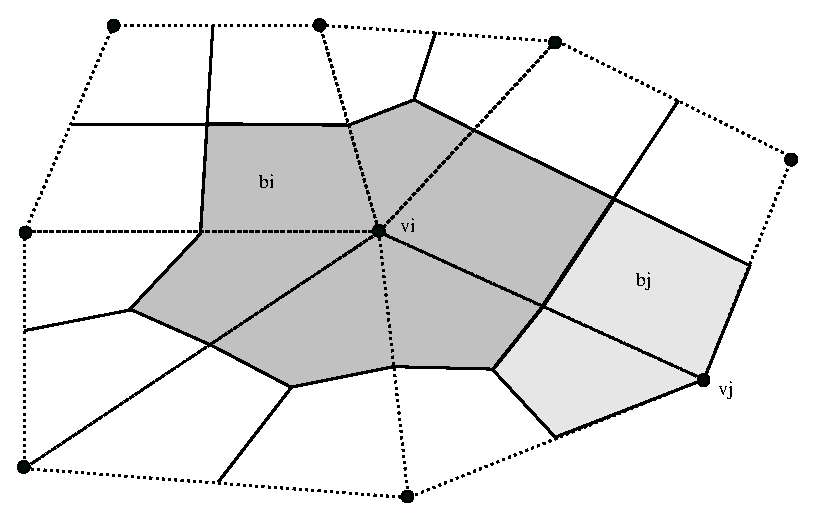
\includegraphics[width=0.4\textwidth]{./EPS/SecMesh2D.eps}},{}]
$E_h^d=\{z_0,\ldots,z_{N_h^d-1}\}$ are the vertices of the mesh
(entities of codimension $d$). 

$x_z$ is the position of $z\in E_h^d$.

$C_h = \{c_0,\ldots,c_{N_h^d-1}\}$ are ``cells'' around each vertex of
the mesh.
\end{window}

$\Omega_c$ is the domain of $c\in C_h$ and $x_c=x_z$ when $c$ is the
cell around $z$.

Define the \textit{discontinuous} test function space:
\begin{align*}
V_h^0 & = \{ v\in L_2(\Omega) \,|\, \forall c\in C_h : v|_{\Omega_c} =
\text{const} \},\\
\tilde{V}_h^0 &= \{ v\in V_h \,|\, \forall z\in E_h^d, x_z\in\Gamma_D : v(x_z)=0\}.
\end{align*}

\end{frame}

\begin{frame}
\frametitle<presentation>{Vertex Centered Finite Volumes (Contd.)}
The discontinuities are located on the \textit{skeleton} which is given by:
\begin{equation*}
\Gamma_h^{\text{int}} = \{\gamma_{e,c,c^\prime} \,|\,
\gamma_{e,c,c^\prime} = \Omega_e \cap \partial\Omega_c \cap
\partial\Omega_{c^\prime} \}
\end{equation*}
and the boundary faces are given by
\begin{equation*}
\Gamma_h^{\text{ext}} = \{\gamma_{e,c} \,|\,
\gamma_{e,c} = \partial\Omega_e \cap \partial\Omega_c \cap
\partial\Omega \}.
\end{equation*}

For $\gamma\in\Gamma_h^{\text{int}}$, $\nu_\gamma(x)$ is
the \textit{unique} unit
normal vector to $\gamma$ in point $x$. 

Similarly, for
$\gamma\in\Gamma_h^{\text{ext}}$, $\nu_\gamma(x)$ is the unit outer
normal vector.

The jump of a function $v\in V_h$ in
$x\in\gamma\in\Gamma_h^{\text{int}}$ given by
\begin{equation*}
[v]_\gamma(x) = \lim_{\varepsilon\to 0-} v(x+\varepsilon \nu_\gamma(x))
-  \lim_{\varepsilon\to 0+} v(x+\varepsilon \nu_\gamma(x))\quad.
\end{equation*}
\end{frame}

\begin{frame}
\frametitle<presentation>{Vertex Centered Finite Volumes (Contd.)}
The discrete problem then reads as follows. Find $u_h\in w_h+\tilde{U}_h^1$ s.t.
\begin{equation}
\underbrace{- \sum_{\gamma\in\Gamma_h^{\text{int}}} \int_\gamma
\nabla u_h \cdot \nu_\gamma \,[v]\diffd s
+ \sum_{\substack{\gamma\in\Gamma_h^{\text{ext}},\\ \gamma\subseteq\Gamma_N}}
\int_\gamma j v \diffd s\quad
- \int_\Omega fv \diffd x}_{= r_h^\text{FE}(u_h,v)} = 0,
\quad \forall v\in \tilde{V}_h^0.
\end{equation}
$\tilde{U}_h^1$ is the linear conforming finite element space and $w_h$ is
defined as before.

Typically, the integrals are evaluated with low order quadrature rules
such as the midpoint rule.

This gives a simple example with non-conforming residual form and
different trial and test functions.
\end{frame}


\paragraph{Cell Centered Finite Volumes}

\begin{frame}
\frametitle<presentation>{Cell Centered Finite Volumes}
Assume that $\mathbb{T}_h$ is either a Delauney
triangulation or a structured cube mesh.

$E^1_h = \{f_0,\ldots,f_{N^1_h-1}\}$ is the set of interior
faces (intersections of two \textit{elements}).

$B^1_h = \{b_0,\ldots,b_{NB^1_h-1}\}$ is the set of exterior faces
(intersections of elements with the domain boundary).

$l,r : E^1_h \to E^0_h$ deliver the ``left'' and ``right'' elements for an
interior face. 

$\nu_f$ denotes the unit normal vector to $f\in E^1_h$ that points from
$l(f)$ to $r(f)$.

Similarly, $l : B^1_h \to E^0_h$ gives the element where $b\in B_h$ is a
face of and $\nu_b$ is the unit outer normal.
\end{frame}

%$\Omega_f$ is the domain of $f\in E_h^1, B_h^1$, $x_f$ is its center.

%$\omega_e = \text{interior}(\overline{\omega_{l(e)}\cup
%\omega_{r(e)}})$ is the domain of the two elements adjacent to $e\in
%E_h$.

%$\omega_b = \omega_{l(e)}$. 

\begin{frame}
\frametitle<presentation>{Cell Centered Finite Volumes (Contd.)}
Define space of \textit{element-wise} constant functions:
\begin{equation*}
W_h^0 = \{  u\in L_2(\Omega) \,|\, \forall e\in E^0_h : u|_{\Omega_e} =
\text{const} \} .
\end{equation*}

The discrete problem then reads
\begin{equation*}
u_h\in W_h^0 \ : \ r_h^\text{CC}(u_h,v) = 0 \quad \forall v\in W^0_h
\end{equation*}
where
\begin{equation*}
\begin{split}
r_h^\text{CC}(u,v) &= \sum_{f\in E^1_h} \int_{\Omega_f}
\frac{u(x_{l(f)}-u(x_{r(f)}))}{\|x_{r(f)}-x_{l(f)}
\|}\,[v]\diffd s
+ \sum_{\substack{b\in B^1_h\\ \Omega_b\subseteq\Gamma_D}} \int_{\Omega_b}
\frac{u(x_{l(b)}-g(x_b))}{\|x_{b}-x_{l(b)}\|}\, v \diffd s \\
& \qquad - \int_\Omega fv \diffd x -
\sum_{\substack{b\in B^1_h\\ \Omega_b\subseteq\Gamma_N}}
\int_{\Omega_b} j v \diffd s .
\end{split}
\end{equation*}

Note that in this formulation there are no essential boundary
conditions. 
\end{frame}

\paragraph{Discontinuous Galerkin}

\begin{frame}
\frametitle<presentation>{Discontinuous Galerkin Finite Element
Method}
Let $k : E^0_h \to \mathbb{N}_0$ be a function that associates an
nonnegative integer with each element.

Define the discrete function space
\begin{equation*}
W_h^k = \{u\in L_2(\Omega) \,|\, \forall e\in E^0_h : u|_{\Omega_e} \in P_{k(e)}\}.
\end{equation*}

For any $x\in\Omega_f, f\in E_h^1$, define the jump of a function
$u\in W_h^k$:
\begin{equation*}
\label{Eq:Jump}
[u]_f(x) = \lim\limits_{\epsilon\to 0-} u(x+\epsilon\nu_f) - 
\lim\limits_{\epsilon\to 0+} u(x+\epsilon\nu_f).
\end{equation*}

For any $x\in\Omega_f, f\in E_h^1$, define the average of a function
$u\in W_h^k$:
\begin{equation*}
\label{Eq:Average}
\langle u\rangle_f(x) = \frac{1}{2}\left(\lim\limits_{\epsilon\to 0-} u(x+\epsilon
\nu_f) +  \lim\limits_{\epsilon\to 0+} u(x+\epsilon
\nu_f)\right ).
\end{equation*}

\end{frame}


\begin{frame}
\frametitle<presentation>{Discontinuous Galerkin Finite Element
Method (Contd.)}
The discrete problem for the OBB method \cite{OBB98} then reads
\begin{equation*}
u_h \in W^k_h \quad : \quad r_h^\text{OBB}(u_h,v) = 0 \qquad \forall v\in W_h^k,
\end{equation*}
where
\begin{equation*}
\begin{split}
r_h^\text{OBB}(u &,v) = \sum_{e\in E_h^0} \int_{\Omega_e} \nabla u\cdot \nabla v
 - fv \, dx \\
&+ \sum_{f\in E^1_h} \int_{\Omega_f} \langle \nabla v\cdot\nu_f\rangle [u]_f
- [v]_f \langle \nabla u\cdot \nu_f\rangle \, ds\\
&+ \sum_{\substack{b\in B^1_h\\\Omega_b\subseteq\Gamma_D}} \int_{\Omega_b} (\nabla v\cdot\nu_f) (u-g)
- v (\nabla u\cdot \nu_f) \, ds + \sum_{\substack{b\in
B^1_h\\\Omega_b\subseteq\Gamma_N}} \int_{\Omega_b} j v \,ds .
\end{split}
\end{equation*}
Note the seperation into volume, skeleton and boundary terms.
\end{frame}


\paragraph{Crouzeix-Raviart}

\begin{frame}
\frametitle<presentation>{Crouzeix-Raviart Element}
Here we use the following discrete spaces:
\begin{align*}
X_h &= \{u\in L_2(\Omega) \,|\, u|_{\Omega_e}\in P_1 \text{ and $u$
continuous at face centers}\},\\
\tilde{X}_h &= \{u\in X_h \,|\, \text{``$u=0$'' on $\Gamma_D$}\}.
\end{align*}

The discrete problem then reads
\begin{equation*}
u_h \in w_h+\tilde{X}_h \quad : \quad r_h^\text{FE}(u_h,v) = 0 \qquad \forall v\in \tilde{X}_h,
\end{equation*}
where again $w_h\in X_h$ such that ``$w_h=g$'' on $\Gamma_D$.
\end{frame}

\paragraph{Mixed Finite Elements}

\begin{frame}
\frametitle<presentation>{Mixed Finite Element Method}
Defining the ``flux'' $\sigma=-\nabla u$ we rewrite problem
\eqref{Eq:DiffusionEquation} as a system of first order equations:
\begin{subequations}
\label{Eq:DiffusionEquationMixedForm}
\begin{align*}
\sigma + \nabla u &= 0 & \text{in }& \Omega\subseteq\mathbb{R}^n,\\
\nabla \cdot \sigma     &= f & \text{in }& \Omega,\\
                      u &= g& \text{on }& \Gamma_D\subseteq\partial\Omega,\\
        \sigma\cdot\nu  &= j& \text{on }& \Gamma_N=\partial\Omega\setminus\Gamma_D.
\end{align*}
\end{subequations}
\end{frame}

\begin{frame}
\frametitle<presentation>{Mixed Finite Element Method (Contd.)}
For the flux we introduce the function space
\begin{subequations}
\begin{align*}
S &= H(\text{div};\Omega) = \{\sigma\in \left(L_2(\Omega)\right)^d \,|\,
\nabla\cdot \sigma \in L_2(\Omega)\},\\
\tilde{S} &= \{\sigma\in S \,|\, \text{``$\sigma\cdot\nu=0$'' on $\Gamma_N$} \}
\end{align*}
\end{subequations}
Note that the Neumann boundary conditions are now the essential
boundary conditions built into the function space.  

Using integration by parts we arrive at the weak formulation of the continuous problem.

Find $(\sigma,u)\in (w+\tilde{S})\times L_2(\Omega)$ s. t.
\begin{align*}
\int\limits_\Omega \sigma\cdot v \, dx  -\int\limits_\Omega
u \, \nabla\cdot v \, dx & =  
-\int\limits_{\Gamma_D} g v\cdot \nu \, ds 
& \forall v &\in \tilde{S}\\
- \int\limits_\Omega \nabla\cdot\sigma \, q \, dx      &= 
- \int\limits_\Omega f q \, ds &
\forall q &\in L_2{\Omega}
\end{align*}
where $w\in S :$ ``$w\cdot\nu = j$'' on $\Gamma_N$.
\end{frame}

\begin{frame}
\frametitle<presentation>{Mixed Finite Element Method (Contd.)}
For discretization use finite dimensional subspaces
of the involved function spaces. 
E.g. the Raviart-Thomas space of lowest order on triangles:
\begin{align*}
S_h &= \left\{\sigma\in\left(L_2(\Omega) \right)^2  \,\Bigl|\, \sigma|_{\Omega_e} =
\left(\begin{array}{l} a_e\\ b_e \end{array}\right) + 
c_e \left(\begin{array}{l} x\\ y \end{array}\right) \quad\forall e\in E^0_h
\right\} .
\end{align*}

Then the discrete problem in residual form reads:
\begin{equation*}
(\sigma_h, u_h) \in (w+\tilde{S}_h)\times W_h^0 : \quad 
r_h^\text{MFE}\left((\sigma_h,u_h),(v,q)\right) = 0 \quad \forall
(v,q) \in \tilde{S}_h\times W_h^0 .
\end{equation*}
with
\begin{equation*}
\begin{split}
r_h^\text{MFE}((\sigma,u)&,(v,q)) = 
\int\limits_\Omega \sigma\cdot v \, dx  -\int\limits_\Omega
u \, \nabla\cdot v \, dx 
 - \int\limits_\Omega \nabla\cdot\sigma \, q \, dx\\ 
&\quad + \int\limits_{\Gamma_D} g v\cdot \nu \, ds + \int\limits_\Omega f q \,
ds .
\end{split}
\end{equation*}
Note: Systems of PDEs lead to tensor product function spaces.
\end{frame}

\subsection{Properties of the Residual Form}

The examples above imply the following properties of $r_h$.

\begin{frame}
\frametitle<presentation>{Properties of the Residual Form}
\begin{Pro}[Splitting]
$r_h$ can be split into element, skeleton and boundary sums
\begin{equation*}
r_h(u,v) = \sum_{e\in E^0_h} r^\text{vol}_{h,e}(u,v) + \sum_{f\in E^1_h} r^\text{skel}_{h,f}(u,v)
+ \sum_{b\in B^1_h} r^\text{bnd}_{h,b}(u,v)
\end{equation*}
$r_h$ can be split into a part depending
on $u$ and a part independent of $u$:
\begin{equation*}
r_h(u,v) = \alpha_h(u,v) + \lambda_h(v) .
\end{equation*}

Together we obtain
\begin{equation}
\begin{split}
r_h(u,v) &= \sum_{e\in E^0_h} \alpha^\text{vol}_{h,e}(u,v) + \sum_{f\in E^1_h} \alpha^\text{skel}_{h,f}(u,v)
+ \sum_{b\in B^1_h} \alpha^\text{bnd}_{h,b}(u,v)\\
&\quad + \sum_{e\in E^0_h} \lambda^\text{vol}_{h,e}(v) + \sum_{f\in E^1_h} \lambda^\text{skel}_{h,f}(v)
+ \sum_{b\in B^1_h} \lambda^\text{bnd}_{h,b}(v) .
\end{split}
\end{equation}
\hfill$\square$
\end{Pro}
\end{frame}

\begin{frame}
\frametitle<presentation>{Properties of the Residual Form (Contd.)}
\begin{Pro}[Linearity]\label{Ass:Linearity}
$r_h$, as well as, $r^\text{vol}_{h,e}$, $r^\text{skel}_{h,f}$ and
$r^\text{bnd}_{h,b}$ are linear in their second
argument.

As a consequence we have $r_h(u,0)=0$.\hfill$\square$
\end{Pro}
\begin{Pro}[Localization]
We assume that the following holds:
\begin{subequations}
\begin{align*}
e&\in E^0_h : & r^\text{vol}_{h,e}(u,v) &= r^\text{vol}_{h,e}(\chi_{\Omega_e} u,\chi_{\Omega_e} v),\\
f&\in E^1_h : & r^\text{skel}_{h,f}(u,v) &=
r^\text{skel}_{h,f}(\chi_{\Omega_{l(f)}\cup\Omega_{r(f)}}
u,\chi_{\Omega_{l(f)}\cup\Omega_{r(f)}} v),\\ 
b&\in B^1_h : & r^\text{bnd}_{h,b}(u,v) &= r^\text{bnd}_{h,b}(\chi_{\Omega_{l(b)}} u,\chi_{\Omega_{l(b)}} v).
\end{align*}
\end{subequations}
where $\chi_\omega(x) : \omega \to \{0,1\}$ is the characteristic function of $\omega$.

This is a consequence of  $r^\text{vol}_{h,e}$, $r^\text{skel}_{h,e}$
and $r^\text{bnd}_{h,e}$ being integrals over an element, an face or a
boundary face. \hfill$\square$
\end{Pro}
\end{frame}


\subsection{Time-dependent Problems}

What about time-dependent problems?

\begin{frame}
\frametitle<presentation>{Time-dependent problems}
Consider time-dependent problems (first order here). We illustrate
only the principal idea.

After semidiscretization in space we obtain a problem of the form
\begin{equation*}
u_h(t)\in U_h : \quad \frac{\partial}{\partial t} m_h(u_h(t),v;t) + q_h(u_h(t),v;t)
= 0 \qquad \forall v\in V_h, t\in\Sigma. 
\end{equation*}
Implicit Euler (e.g.) then leads to: Find $u_h^{k+1}\in U_h$ s.t.
\begin{equation*}
\underbrace{m_h(u_h^{k+1},v;t^{k+1}) - m_h(u_h^{k},v;t^k) + \Delta
t^{k}q_h(u_h^{k+1},v;t^{k+1})}_{r_h^\text{IE}(u_h,v)}  = 0
\quad v\in V_h.
\end{equation*}

Explicit Euler (e.g.) leads to: Find  $u_h^{k+1}\in U_h$ s.t.
\begin{equation*}
\underbrace{m_h(u_h^{k+1},v;t^{k+1}) - m_h(u_h^{k},v;t^k) + \Delta
t^{k}q_h(u_h^{k},v;t^{k})}_{r_h^\text{EE}(u_h,v)}  = 0
\quad v\in V_h.
\end{equation*}
Higher-order time discretizations lead to similar problems.

Explicit schemes may lead to easily invertible algebraic systems.
\end{frame}

\cleardoublepage

%%%%%%%%%%%%%%%%%%%%%%%%%%%%%%%%%%%%%%%%%%%%%%%%%%%%%%%%%%%%
%%%%%%%%%%%%%%%%%%%%%%%%%%%%%%%%%%%%%%%%%%%%%%%%%%%%%%%%%%%%
%%%%%%%%%%%%%%%%%%%%%%%%%%%%%%%%%%%%%%%%%%%%%%%%%%%%%%%%%%%%
\section{Finite-dimensional Function Spaces}\label{Sec:General}
%%%%%%%%%%%%%%%%%%%%%%%%%%%%%%%%%%%%%%%%%%%%%%%%%%%%%%%%%%%%
%%%%%%%%%%%%%%%%%%%%%%%%%%%%%%%%%%%%%%%%%%%%%%%%%%%%%%%%%%%%
%%%%%%%%%%%%%%%%%%%%%%%%%%%%%%%%%%%%%%%%%%%%%%%%%%%%%%%%%%%%

Our general PDE problem includes the definition of unconstrained and
constrained finite-dimensional (i.~e.~discrete) function spaces. In
this section we will define such spaces in a general way. 

\subsection{Unconstrained Spaces}

\begin{frame}
\frametitle<presentation>{Finite-dimensional Function Spaces}
$\Omega\subset\mathbb{R}^n$, $n\geq 1$, is a domain, 
$\mathbb{T}_h$ a grid partitioning the domain $\Omega$.

\begin{Def}[Finite-dimensional function space]\label{Def:Vh}
\begin{equation*}\label{Eq:GenericFESpace}
\begin{split}
U_h(\mathbb{T}_h) &= \Biggl\{ u_h(x) : \bigcup_{e\in E_h^0}\Omega_e
 \to \mathbb{K}^m\,\Bigg| \\
&\quad u_h(x) = \sum_{e\in E_h^0}\sum_{i=0}^{k(e)-1} (\mathbf{u})_{g(e,i)}
\, \pi_e(\hat{x}) \, \hat\phi_{e,i}(\hat{x}) \, \chi_e(x); \, \hat{x}=\mu_e^{-1}(x) 
 \Biggr\}
\end{split}
\end{equation*}
defines a general finite-dimensional function space of element-wise
continuous functions.\hfill$\square$ 
\end{Def}
\end{frame}

The individual components in this definition are:
\begin{frame}
\frametitle<presentation>{Finite-dimensional Function Spaces (Contd.)}
\begin{itemize}
\item $\mathbb{K}=\mathbb{R}$ or $\mathbb{K}=\mathbb{C}$.
  $m\geq 1$ denotes vector-valued function spaces. 
\item $\hat\Omega_e$ is the \textit{reference element} associated with
element $e\in E_h^0$. $\mu_e : \overline{\hat\Omega}_e \to
  \overline{\Omega}_e$ maps the reference element to $\Omega$.
\item $\hat\Phi_e
  = \left\{\hat\phi_{e,i}: \overline{\hat\Omega}_e \to \mathbb{R}^{m'}\,|\,0\leq
  i < k(e)\right\}$ is 
  the set of \textit{local basis functions} for element $e$.
\item $\pi_e(\hat{x})\in\mathbb{R}^{m\times m'}$ is a
  transformation. A non-trivial example is the Piola
  transformation \cite{BrezziFortin}
\begin{equation*}
\pi_e(\hat{x}) = \frac{1}{\text{det}\  \mu_e(\hat{x})} \nabla \mu_e(\hat{x})
\end{equation*}
where $\nabla \mu_e$ denotes the Jacobian of the map $\mu_e$. For most
finite element spaces $\pi_e$ is just the identity and we have $m'=m$.
\item $g : L \to \mathbb{N}$, $L=\left\{ (e,i)\in E_h^0 \times
  \mathbb{N} \,|\, 0\leq i < k(e)\right\}$ is the \textit{local to global map}
  and $\mathcal{I}_{U_h} = \text{im}\,g$ is the associated \textit{global index set}.
\item $\mathbf{u}\in \mathbf{U}=\mathbb{K}^{\mathcal{I}_{U_h}}$ is a coefficient vector.
\end{itemize}
\end{frame}

\begin{frame}
\frametitle<presentation>{Global Basis}
For $j\in \mathcal{I}_{U_h}$ we define the \textit{global basis function}
\begin{equation*}
U_h \ni \phi_j(x) = \sum_{(e,i)\in l(j)} \pi_e(\hat{\mu_e^{-1}(x)}) \,
\hat\phi_{e,i}(\mu_e^{-1}(x)) \, \chi_e(x)
\end{equation*} 
and $l(j) = \left\{ (e,i)\in L \,|\, g(e,i)=j \right\}$.
With that we have
\begin{align}
\Phi_{U_h} &= \{\phi_i \,|\, i\in \mathcal{I}_{U_h}\}, & U_h &= \text{span}\ \Phi_{U_h}.
\end{align}
and the finite element isomorphism
\begin{align}\label{Eq:FiniteElementIsomorphism}
\text{FE}_{\Phi_{U_h}} &: \mathbf{U} \to
U_h, & \text{FE}_{\Phi_{U_h}}(\mathbf{u})
&= \sum_{i\in\mathcal{I}_{U_h}} (\mathbf{u})_i \phi_i \ . 
\end{align} 

Definition \ref{Def:Vh} allows for functions that are
\textit{discontinuous} at element boundaries. 

If limits on the skeleton $\Gamma_h = \Omega\setminus \bigcup_ {e\in
  E_h^0} \Omega_e$ coincide, a function may be extended to 
$\left(C^0(\Omega)\right)^m$.
\end{frame}

\subsection{Constrained Spaces}

As we have seen we often have the situation that problems have to be solved in a
subspace $\tilde{U}_h\subset U_h$ or even an affine subspace
$w_h+\tilde{U}_h$, where $w_h\in U_h$.

\paragraph{Basis transformation} 

\begin{frame}
\frametitle<presentation>{Basis Transformation}
\begin{Def}[Basis Transformation] Consider an alternative basis
$\Phi_{U_h}'=\{\phi_i'\,|\, i\in \mathcal{I}_{U_h}\}$ of $U_h$
obtained by
\begin{equation}
\phi_i' = \sum_{j\in\mathcal{I}_{U_h}}
\left(\mathbf{T}_{U_h}\right)_{i,j} \phi_j, \qquad i\in \mathcal{I}_{U_h}.
\end{equation}
$\mathbf{T}_{U_h}$ is the \textit{transformation matrix}.\hfill$\square$
\end{Def}
For $\mathbf{U}'=\mathbb{K}^{\mathcal{I}_{U_h}}$ we have the isomorphism
$\text{FE}_{\Phi_{U_h}'}(\mathbf{u}') = \sum_{i\in\mathcal{I}_{U_h}}
(\mathbf{u}')_i \phi_i'$ and get
\begin{equation}
\begin{split}
u_h &= \text{FE}_{\Phi_{U_h}'}(\mathbf{u}') = 
\sum_{j\in\mathcal{I}_{\tilde{U}_h}} (\mathbf{u}')_j \phi'_j = 
\sum_{j\in\mathcal{I}_{U_h}} (\mathbf{u}')_j \left (
\sum_{i\in\mathcal{I}_{U_h}}
\left(\mathbf{T}_{U_h}\right)_{j,i} \phi_i \right)\\
&= \sum_{i\in \mathcal{I}_{U_h}} \left (\sum_{j\in\mathcal{I}_{U_h}}
\left(\mathbf{T}^T_{U_h}\right)_{i,j} (\mathbf{u}')_j \right ) \phi_i
= \text{FE}_{\Phi_{U_h}}\left( \mathbf{T}^T_{U_h} \mathbf{u}' \right) .
\end{split}
\end{equation}
\end{frame}

\paragraph{Splitting and Subspaces} 

\begin{frame}
\frametitle<presentation>{Splitting and Subspaces}
Subspaces are introduced by a splitting of
the index set into unconstrained and constrained indices:
\begin{equation*}
\mathcal{I}_{U_h} = \tilde{\mathcal{I}}_{U_h} \cup
\bar{\mathcal{I}}_{U_h}, \qquad  \tilde{\mathcal{I}}_{U_h} \cap
\bar{\mathcal{I}}_{U_h} = \emptyset.
\end{equation*}
With respect to this splitting we define the subspaces
\begin{align*}
\tilde{U}_h' &= \text{span}\ \{\phi_i'\,|\,
i\in\tilde{\mathcal{I}}_{U_h}\}, &
\bar{U}_h' &= \text{span}\ \{\phi_i'\,|\,
i\in\bar{\mathcal{I}}_{U_h}\}
\end{align*}
and the corresponding coefficient spaces
\begin{align*}
\tilde{\mathbf{U}}' &=
\mathbb{K}^{\tilde{\mathcal{I}}_{U_h}}, &
\bar{\mathbf{U}}' &=
\mathbb{K}^{\bar{\mathcal{I}}_{U_h}}.
\end{align*}

$\tilde{U}_h := \tilde{U}_h'\subseteq U_h$ is the desired subspace of
$U_h$ where we want to solve the constrained problem.
\end{frame}


\begin{frame}
\frametitle<presentation>{Simplified Transformation Matrix}
The transformation matrix $\mathbf{T}_{U_h}$ is written in block
form w.r.t. the splitting:
\begin{equation*}
\mathbf{T}_{U_h} = \left(\begin{array}{cc}
\mathbf{T}_{\tilde{U}_h,\tilde{U}_h} & \mathbf{T}_{\tilde{U}_h,\bar{U}_h}\\
\mathbf{T}_{\bar{U}_h,\tilde{U}_h} & \mathbf{T}_{\bar{U}_h,\bar{U}_h}
\end{array}\right) .
\end{equation*}
We show below that it suffices to consider transformations of the form
\begin{equation}\label{Eq:StructureTransformation}
\mathbf{T}_{U_h} = \left(\begin{array}{cc}
\mathbf{I} & \mathbf{T}_{\tilde{U}_h,\bar{U}_h}\\
\mathbf{0} & \mathbf{I}
\end{array}\right)
\end{equation}
which means transformations have the form
\begin{equation*}
\phi_i' = \phi_i + \sum_{j\in\bar{\mathcal{I}}_{U_h}}
\left(\mathbf{T}_{\tilde{U}_h,\bar{U}_h}\right)_{i,j} \phi_j, \qquad i\in \tilde{\mathcal{I}}_{U_h}.
\end{equation*}
The $\tilde{\mathcal{I}}_{U_h} \times \bar{\mathcal{I}}_{U_h}$  matrix
$\mathbf{T}_{\tilde{U}_h,\bar{U}_h}$ will usually be very sparse (or
even zero).
\end{frame}

\paragraph{Restrictions} 

\begin{frame}
\frametitle<presentation>{Restriction Operators}
Below we will make use of the following restriction operators
\begin{align*}
\mathbf{R}_{\tilde{\mathbf{U}}',\mathbf{U}'} &: \mathbf{U}' \to \tilde{\mathbf{U}}', & 
(\mathbf{R}_{\tilde{\mathbf{U}}',\mathbf{U}'}\mathbf{u}')_i &= 
(\mathbf{u}')_i \quad \forall i\in \tilde{\mathcal{I}}_{U_h},\\
\mathbf{R}_{\bar{\mathbf{U}}',\mathbf{U}'} &: \mathbf{U}' \to \bar{\mathbf{U}}', & 
(\mathbf{R}_{\bar{\mathbf{U}}',\mathbf{U}'}\mathbf{u}')_i &= 
(\mathbf{u}')_i \quad \forall i\in \bar{\mathcal{I}}_{U_h}.
\end{align*}

Note that $\mathbf{Q}_{\tilde{\mathbf{U}}}
= \mathbf{R}_{\tilde{\mathbf{U}}',\mathbf{U}'}^T \mathbf{R}_{\tilde{\mathbf{U}}',\mathbf{U}'}$
is an orthogonal projection.

It can be used to project a function from $U_h$ to $\tilde{U}_h$ as
follows:
\begin{align*}
P_h &: U_h \to \tilde{U}_h, & P_h  =
FE_{\Phi_h'} \circ \mathbf{Q}_{\tilde{\mathbf{U}}} \circ
FE_{\Phi_h'}^{-1} .
\end{align*}

The projection $P_h$ will play a major role below.
\end{frame}

\subsection{Examples of Constrained Spaces}

\paragraph{Dirichlet Boundary Conditions}

\begin{frame}
\frametitle<presentation>{Dirichlet Boundary Conditions}
$U_h^1$ :  piecewise-linear, conforming finite
element functions.

$\tilde{U}_h^1 = \{u\in U_h^1 \,|\, \text{``$u(x)=0$'' for
$x\in \Gamma_D$}\}$.

Then just set 
\begin{align*}
\bar{\mathcal{I}}_{U_h} &= \{i\in \mathcal{I}_{U_h} \,|\,
x_{z_i}\in\Gamma_D\}, &
\tilde{\mathcal{I}}_{U_h} =  \mathcal{I}_{U_h}\setminus\bar{\mathcal{I}}_{U_h}
\end{align*}
and
\begin{equation*}
\phi_i' = \phi_i \qquad i\in \tilde{\mathcal{I}}_{U_h}.
\end{equation*}

Obviously, $\mathbf{T}_{\tilde{U}_h,\bar{U}_h}=\mathbf{0}$ in this case.
\end{frame}

\paragraph{Hanging Nodes}

Consider a mesh obtained from non-conforming refinement.

\begin{frame}
\frametitle<presentation>{Hanging Nodes}
\begin{columns}
\begin{column}{0.6\textwidth}
$U_h^1$ now is the space of piecewise linear functions with degrees of
freedom in \textit{all} vertices of the mesh. \\
\medskip
To obtain the subspace $\tilde{U}_h^1 = U_h^1 \cap C^0(\Omega)$ we set 
\begin{align*}
\bar{\mathcal{I}}_{U_h} &= \{i\in \mathcal{I}_{U_h} \,|\, \text{$z_i$ is a
hanging node} \}, \\
\tilde{\mathcal{I}}_{U_h} &=  \mathcal{I}_{U_h}\setminus\bar{\mathcal{I}}_{U_h}.
\end{align*}
\end{column}
\mode<presentation>{
\begin{column}{0.4\textwidth}
\psfrag{0}{{\tiny $0$}}
\psfrag{1}{{\tiny $1$}}
\psfrag{h}{{\tiny $\frac12$}}
\psfrag{vi}{$v_i$}
\psfrag{vj}{$v_j$}
\psfrag{vk}{$v_k$}
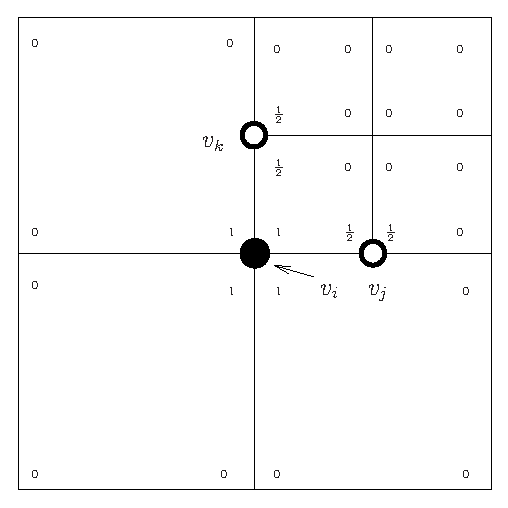
\includegraphics[width=\textwidth]{./EPS/function3.eps}
\end{column}}
\end{columns}
\mode<article>{
\begin{figure}
\begin{center}
\psfrag{0}{{\tiny $0$}}
\psfrag{1}{{\tiny $1$}}
\psfrag{h}{{\tiny $\frac12$}}
\psfrag{vi}{$v_i$}
\psfrag{vj}{$v_j$}
\psfrag{vk}{$v_k$}
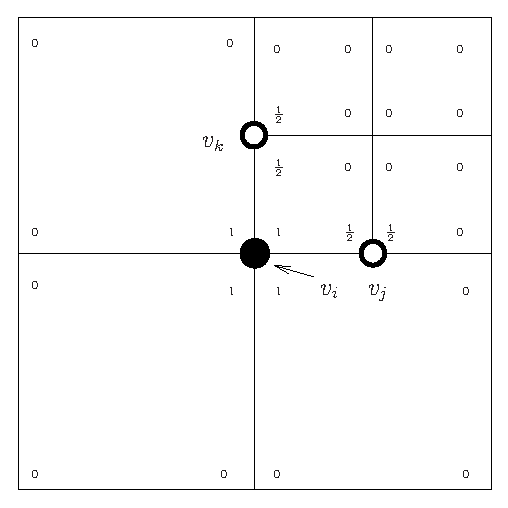
\includegraphics[width=0.5\textwidth]{./EPS/function3.eps}
\end{center}
\caption{Non-conforming refinement and piecewise linear finite elements.}
\end{figure}}
For the vertex $i$ in the figure we obtain, e.~g., the basis function
\begin{equation*}
\phi_i' = \phi_i + \frac12 \phi_j + \frac12 \phi_k .
\end{equation*}
\end{frame}


\paragraph{Pure Neumann Problem}

\begin{frame}
\frametitle<presentation>{Pure Neumann Problem}
We wish to solve
\begin{align*}
                -\Delta u &= f& \text{in }& \Omega\subseteq\mathbb{R}^n,\\
     - \nabla u\cdot\nu   &= j& \text{on }& \partial\Omega
\end{align*}
where $\int_{\partial\Omega} j \, ds = \int_\Omega f \, dx$.

Again, consider $U_h^1$, the piecewise-linear, conforming finite
element functions.

Then $u$ is only defined up to a constant and we wish to solve in
\begin{equation*}
\tilde{U}^1_h = \left\{u \in U^1_h \,\Biggl |\, \int_\Omega u \, dx = 0\right\}.
\end{equation*}

Set $\bar{\mathcal{I}}_{U_h}=\{0\}$, $\tilde{\mathcal{I}}_{U_h}
= \mathcal{I}_{U_h}\setminus\{0\}$ and
\begin{equation*}
\phi_i' = \phi_i - \frac{\int_\Omega\phi_i\, dx}{\int_\Omega\phi_0\,
dx} \phi_0, \qquad \forall i\in\tilde{\mathcal{I}}_{U_h}.
\end{equation*}
\end{frame}

\paragraph{Other Situations Where Constraints Occur}

\begin{frame}
\frametitle<presentation>{Other Constraints}
In the same way we can also treat
\begin{itemize}
\item Varying polynomial degree in conforming finite elements
($p$-refinement).
\item Combination of $p$-refinement, non-conforming refinement and essential
boundary conditions.
\item Non-conforming refinement in mixed finite elements.
\item Periodic boundary conditions.
\item Constraints in parallel overlapping Schwarz methods.
\end{itemize}
\end{frame}


\subsection{Function Space Composition}

\begin{frame}
\frametitle<presentation>{Function Space Composition}
For systems we need composite function spaces.

Given $k>1$ function spaces $U_0, \ldots, U_{k-1}$ we define the
composite function space 
\begin{equation}
U = U_0 \times U_1 \times \ldots \times U_{k-1} .
\end{equation}

If all component spaces are the same we can also write
\begin{equation}
U = V^k
\end{equation}

This can be done recursively. E.g. for solving the Stokes equation
in dimension $d$ using Taylor-Hood elements we would require
\begin{equation*}
U_h^\text{TH} = \left( U_h^2\right)^d \times U_h^1
\end{equation*}

Composite function spaces can be visualized as a tree:
\begin{minipage}[c]{0.2\textwidth}
\psfrag{P1}{$U_h^1$} 
\psfrag{P2}{$U_h^2$} 
\psfrag{TH}{$U_h^\text{TH}$} 
\psfrag{Vel}{$U_h^\text{V}$} 
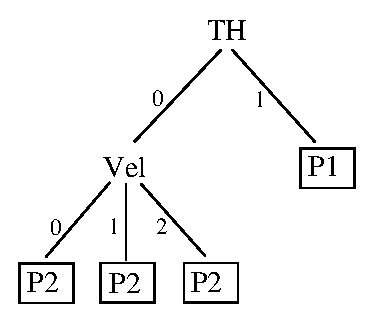
\includegraphics[width=\textwidth]{./EPS/THBaum.eps}
\end{minipage}

\end{frame}

\cleardoublepage

%%%%%%%%%%%%%%%%%%%%%%%%%%%%%%%%%%%%%%%%%%%%%%%%%%%%%%%%%%%%
%%%%%%%%%%%%%%%%%%%%%%%%%%%%%%%%%%%%%%%%%%%%%%%%%%%%%%%%%%%%
%%%%%%%%%%%%%%%%%%%%%%%%%%%%%%%%%%%%%%%%%%%%%%%%%%%%%%%%%%%%
\section{Discrete Functions in \texttt{dune-pdelab}}
%%%%%%%%%%%%%%%%%%%%%%%%%%%%%%%%%%%%%%%%%%%%%%%%%%%%%%%%%%%%
%%%%%%%%%%%%%%%%%%%%%%%%%%%%%%%%%%%%%%%%%%%%%%%%%%%%%%%%%%%%
%%%%%%%%%%%%%%%%%%%%%%%%%%%%%%%%%%%%%%%%%%%%%%%%%%%%%%%%%%%%

\cleardoublepage

%%%%%%%%%%%%%%%%%%%%%%%%%%%%%%%%%%%%%%%%%%%%%%%%%%%%%%%%%%%%
%%%%%%%%%%%%%%%%%%%%%%%%%%%%%%%%%%%%%%%%%%%%%%%%%%%%%%%%%%%%
%%%%%%%%%%%%%%%%%%%%%%%%%%%%%%%%%%%%%%%%%%%%%%%%%%%%%%%%%%%%
\section{Algebraic Formulation}
%%%%%%%%%%%%%%%%%%%%%%%%%%%%%%%%%%%%%%%%%%%%%%%%%%%%%%%%%%%%
%%%%%%%%%%%%%%%%%%%%%%%%%%%%%%%%%%%%%%%%%%%%%%%%%%%%%%%%%%%%
%%%%%%%%%%%%%%%%%%%%%%%%%%%%%%%%%%%%%%%%%%%%%%%%%%%%%%%%%%%%

\subsection{Solution of the Unconstrained Problem}

\paragraph{Unconstrained Problem in Original Basis}

\begin{frame}
\frametitle<presentation>{Unconstrained Problem in Original Basis}
We recall the unconstrained problem in weighted residual form:
\begin{equation}
u_h\in U_h\ : \qquad r_h(u_h,v) = 0 \qquad \forall
v\in V_h .
\end{equation}

Solving it in the original basis
reduces to the solution of a nonlinear algebraic problem:
\begin{equation}
\begin{split}
\mathbf{u}\in\mathbf{U} : \qquad
& r_h\left(\text{FE}_{\Phi_{U_h}}(\mathbf{u}),\psi_i\right) = 0, \quad
i\in\mathcal{I}_{V_h} \\
\Leftrightarrow \  & \mathcal{R}(\mathbf{u}) = \mathbf{0}
\end{split}
\end{equation}
where we introduced the nonlinear residual map $\mathcal{R} :
\mathbf{U} = \mathbb{K}^{\mathcal{I}_{V_h}} \to \mathbb{K}^{\mathcal{I}_{V_h}}$ which is defined as 
\begin{equation}
\left(
\mathcal{R}(\mathbf{u})\right)_i =
r_h(\text{FE}_{U_h}(\mathbf{u}),\psi_i).
\end{equation}
$\Phi_{V_h} = \{\psi_i\,|\, i\in\mathcal{I}_{V_h}\}$ is the basis of $V_h$.  
\end{frame}

\paragraph{Unconstrained Problem in Transformed Basis}

\begin{frame}
\frametitle<presentation>{Unconstrained Problem in Transformed Basis}
We may also solve the unconstrained problem 
in the transformed basis for trial and test space:
\begin{equation}\label{Eq:TransformedUnconstrainedProblem}
\begin{split}
\mathbf{u}'\in\mathbf{U}' : \qquad 
& r_h\left(\text{FE}_{\Phi'_{U_h}}(\mathbf{u}'),\psi_i'\right) = 0, \quad
i\in\mathcal{I}_{V_h}\\
\Leftrightarrow \  &
r_h\left(\text{FE}_{\Phi_{U_h}}(\mathbf{T}^T_{U_h}\mathbf{u}'),
\sum_{j\in\mathcal{I}_{V_h}}\left(\mathbf{T}_{V_h}\right)_{i,j}\psi_j\right) = 0, \quad
i\in\mathcal{I}_{V_h}\\
\Leftrightarrow \  &
\sum_{j\in\mathcal{I}_{V_h}} \left(\mathbf{T}_{V_h}\right)_{i,j} 
r_h\left(\text{FE}_{\Phi_{U_h}}(\mathbf{T}^T_{U_h}\mathbf{u}'),
\psi_j\right) = 0, \quad
i\in\mathcal{I}_{V_h}\\
\Leftrightarrow \  &
\mathbf{T}_{V_h} \mathcal{R}\left(\mathbf{T}^T_{U_h}\mathbf{u}'\right)
= \mathbf{0} .
\end{split}
\end{equation}
Used linearity of residual form with respect to the second argument.

Requires simple matrix multiplication.
\end{frame}

\paragraph{Newton solver}

Use Newton's method to solve the algebraic problem.

\begin{frame}
\frametitle<presentation>{Newton Solver}
Let a current iterate $\mathbf{u}_k'$ be given. 

We seek an update $\mathbf{z}'_k$ such that $\mathbf{u}'_{k+1} = \mathbf{u}_k'
+ \mathbf{z}'_k$ and linearize:
\begin{equation*}
\mathbf{T}_{V_h}\mathcal{R}\left(\mathbf{T}^T_{U_h}\mathbf{u}'_{k+1}\right) \approx 
\mathbf{T}_{V_h}\mathcal{R}\left(\mathbf{T}^T_{U_h}\mathbf{u}'_{k}\right) +
\mathbf{T}_{V_h}\nabla\mathcal{R}\left(\mathbf{T}^T_{U_h}\mathbf{u}'_{k}\right) 
\mathbf{T}^T_{U_h} \mathbf{z}'_{k} = \mathbf{0} .
\end{equation*}

A linear system for the update is 
\begin{equation}\label{eq:UnconstrainedUpdate}
\mathbf{T}_{V_h}\nabla\mathcal{R}\left(\mathbf{T}^T_{U_h}\mathbf{u}'_{k}\right) 
\mathbf{T}^T_{U_h} \mathbf{z}'_{k} = -
\mathbf{T}_{V_h}\mathcal{R}\left(\mathbf{T}^T_{U_h}\mathbf{u}'_{k}\right) .
\end{equation}

$\nabla\mathcal{R}\left(\mathbf{u}_{k}\right)$ denotes the
Jacobian matrix of the map $\mathcal{R}$. 

Multiplying the update equation with $\mathbf{T}^T_{U_h}$ from the left yields
\begin{equation}\label{eq:OriginalUpdate}
\mathbf{T}^T_{U_h}\mathbf{u}'_{k+1} = \mathbf{T}^T_{U_h}\mathbf{u}_k' +
\mathbf{T}^T_{U_h}\mathbf{z}'_k .
\end{equation}

Setting $\mathbf{u}_{k} := \mathbf{T}^T_{U_h}\mathbf{u}_k'$ allows us
now to write the Newton scheme with respect to the original basis.
\end{frame}


\begin{frame}
\frametitle<presentation>{Newton Solver (Contd.)}
\begin{Alg}[Newton's method for unconstrained problem]
Given the initial guess $\mathbf{u}_{0}$ iterate until convergence
\begin{enumerate}[i)]
\item Compute residual:
  $\mathbf{r}_k=-\mathcal{R}\left(\mathbf{u}_{k}\right)$.
\item Transform residual: $\mathbf{r}_k' = \mathbf{T}_{V_h}
  \mathbf{r}_k$.
\item Solve update equation:
  $\mathbf{T}_{V_h}\nabla\mathcal{R}\left(\mathbf{u}_{k}\right)  
\mathbf{T}^T_{U_h} \mathbf{z}'_{k} =  \mathbf{r}_k'$.
\item Transform update: $\mathbf{z}_{k} =
  \mathbf{T}^T_{U_h}\mathbf{z}'_k$.
\item Update: $\mathbf{u}_{k+1} = \mathbf{u}_k
+ \mathbf{z}_k$. \hfill$\square$
\end{enumerate}
\end{Alg}

Two applications of the basis transformation, for the
residual and the update, are necessary in steps ii) and iv).

These transformations are cheap due to the structure of the
transformation.

In step (iii) the \textit{transformed}
Jacobian system is required.

\textit{All these transformations are done generically by PDELab}!
\end{frame}

\subsection{Solution of Constrained Problem}

We now turn to the constrained problem.

\paragraph{Reformulation in unconstrained space}

\begin{frame}
\frametitle<presentation>{Reformulation in unconstrained space}
We recall the constrained problem in weighted residual form:
\begin{equation}\label{Eq:ConstrainedProblem}
u_h\in w_h + \tilde{U}_h\ : \qquad r_h(u_h,v) = 0 \quad \forall
v\in \tilde{V}_h .
\end{equation}

This problem can be reformulated in the unconstrained space by adding
a constrained equation:
\begin{Prp}
Let $P_h : U_h \to \tilde{U}_h$ be a projection (i.~e.~$P_h^2 = P_h$)
and assume that the affine shift is such that $P_h w_h = 0$. Then 
\begin{equation}\label{Eq:ConstrainedProblemReformII}
u_h\in U_h\ : \qquad \left\{\begin{array}{ll}
r_h(u_h,v) = 0 \quad \forall v\in \tilde{V}_h\\
(I-P_h)u_h = w_h
\end{array}\right. 
\end{equation}
is equivalent to \eqref{Eq:ConstrainedProblem}.

\mode<article>{
\textit{Proof}. Assume that \eqref{Eq:ConstrainedProblem} holds and
$P_h w_h = 0$. Since $u_h$ solves \eqref{Eq:ConstrainedProblem}
the first equation in \eqref{Eq:ConstrainedProblemReformII} clearly holds.
Moreover, we have $u_h = w_h + \tilde{u}_h$ with $\tilde{u}_h\in
\tilde{U}_h$ which allows us to write $u_h = w_h + P_h v_h$ for some
$v_h\in U_h$. When we can prove that $v_h=u_h$ we obtain the desired
$(I-P_h)u_h = w_h$. We now show that $v_h=u_h$:
Applying $P_h$ to both sides of the identity $u_h = w_h + P_h v_h$ yields
$P_h u_h = P_h w_h + P_h^2 v_h$. Using $P_h w_h = 0$ and $P_h^2 = P_h$
yields $P_h u_h = P_h v_h$. Thus we may identify $v_h$ and $u_h$ as
$v_h$ was arbitrary.\\
Assume now that \eqref{Eq:ConstrainedProblemReformII} holds. The first
equation of \eqref{Eq:ConstrainedProblemReformII} is the same as 
\eqref{Eq:ConstrainedProblem}. From the
second equation we conclude $u_h = w_h + P_h u_h$, i.~e.~ $u_h\in w_h
+ \tilde{U}_h$.} \hfill$\square$
\end{Prp}
\end{frame}

\paragraph{Reformulated Problem in Coefficient Space} 

We now seek to solve problem
\eqref{Eq:ConstrainedProblemReformII} in coefficient space. 

\begin{frame}
\frametitle<presentation>{Reformulated Problem in Coefficient Space}
The projection $P_h$ is taken from the follwing commutative diagram:
\begin{equation*}
\begin{CD}
U_h @>{P_h = \text{FE}_{\Phi'_{U_h}}
\mathbf{R}^T_{\tilde{\mathbf{U}}',\mathbf{U}'}
\mathbf{R}_{\tilde{\mathbf{U}}',\mathbf{U}'} 
\text{FE}_{\Phi'_{U_h}}^{-1}}>> \tilde{U}_h\\
@A{\text{FE}_{\Phi'_{U_h}}}AA @AA{\text{FE}_{\Phi'_{U_h}}
\mathbf{R}^T_{\tilde{\mathbf{U}}'\mathbf{U}'}}A\\
\mathbf{U}' @>{\qquad\mathbf{R}_{\tilde{\mathbf{U}}',\mathbf{U}'}\qquad}>> \tilde{\mathbf{U}}' 
\end{CD}
\end{equation*}

\begin{Prp}
Using this definition of $P_h$ the reformulated constrained
problem \eqref{Eq:ConstrainedProblemReformII} in coefficient space reads
\begin{equation}\label{Eq:ConstrainedProblemInCoefficientSpace}
\mathbf{u}'\in\mathbf{U}' : \qquad \left\{\begin{array}{rcl}
\mathbf{S}_{\tilde{\mathbf{V}}'}
\mathcal{R}\left(\mathbf{T}^T_{U_h}\mathbf{u}'\right)
& = & \mathbf{0}\\
\mathbf{R}_{\bar{\mathbf{U}}',\mathbf{U}'} \mathbf{u}' & = & \mathbf{w}'
\end{array}\right.
\end{equation}
with $\mathbf{S}_{\tilde{\mathbf{V}}'}=\mathbf{R}_{\tilde{\mathbf{V}}',\mathbf{V}'} +
\mathbf{T}_{\tilde{V}_h,\bar{V}_h}\mathbf{R}_{\bar{\mathbf{V}}',\mathbf{V}'}$
and $w_h =
FE_{\Phi_{U_h}'}(\mathbf{R}_{\bar{\mathbf{U}}',\mathbf{U}'}^T\mathbf{w}')$.
\hfill$\square$
\end{Prp}
\end{frame}

The idea in this formulation is that with respect to the transformed
basis the affine shift (for Dirichlet boundary conditions) can be
``encoded'' in the constrained degrees of freedom
$\mathbf{R}_{\bar{\mathbf{U}}',\mathbf{U}'} \mathbf{u}'$. This is
possible because the subspace $\tilde{U}_h$ is the image
of the unconstrained degrees of freedom
$\mathbf{R}_{\tilde{\mathbf{U}}',\mathbf{U}'} \mathbf{u}'$ 
and the decomposition is orthogonal
(i.~e.~$\mathbf{R}^T_{\bar{\mathbf{U}}',\mathbf{U}'}
\mathbf{R}_{\bar{\mathbf{U}}',\mathbf{U}'}$ and
$\mathbf{R}^T_{\tilde{\mathbf{U}}',\mathbf{U}'}
\mathbf{R}_{\tilde{\mathbf{U}}',\mathbf{U}'}$ are orthogonal
projections). 


\begin{frame}
\frametitle<presentation>{Proof of Proposition}
The second equation is seen as follows:
\begin{equation}\label{Eq:SideConditionCoefficient}
\begin{split}
&(I-P_h) u_h = w_h \\
\Leftrightarrow \quad & 
\left(\text{FE}_{\Phi'_{U_h}}\text{FE}_{\Phi'_{U_h}}^{-1}
- \text{FE}_{\Phi'_{U_h}}
\mathbf{R}^T_{\tilde{\mathbf{U}}',\mathbf{U}'}
\mathbf{R}_{\tilde{\mathbf{U}}',\mathbf{U}'} 
\text{FE}_{\Phi'_{U_h}}^{-1}\right)\text{FE}_{\Phi'_{U_h}}\mathbf{u}'
= \text{FE}_{\Phi'_{U_h}}
\mathbf{R}^T_{\bar{\mathbf{U}}',\mathbf{U}'} \mathbf{w}'\\
\Leftrightarrow \quad &
\left( \mathbf{I} - \mathbf{R}^T_{\tilde{\mathbf{U}}',\mathbf{U}'}
\mathbf{R}_{\tilde{\mathbf{U}}',\mathbf{U}'}\right) \mathbf{u}' =
\mathbf{R}^T_{\bar{\mathbf{U}}',\mathbf{U}'} \mathbf{w}' \\
\Leftrightarrow \quad &
\mathbf{R}^T_{\bar{\mathbf{U}}',\mathbf{U}'}
\mathbf{R}_{\bar{\mathbf{U}}',\mathbf{U}'} \mathbf{u}' =
\mathbf{R}^T_{\bar{\mathbf{U}}',\mathbf{U}'} \mathbf{w}'\\
\Leftrightarrow \quad &
\mathbf{R}_{\bar{\mathbf{U}}',\mathbf{U}'} \mathbf{u}' = \mathbf{w}' .
\end{split}
\end{equation}
\end{frame}

\begin{frame}
\frametitle<presentation>{Proof of Proposition (Contd.)}
For the first equation in \eqref{Eq:ConstrainedProblemReformII} 
we proceed as in \eqref{Eq:TransformedUnconstrainedProblem}
\begin{equation}\label{Eq:TransformedConstrainedProblem2}
\begin{split}
\mathbf{u}'\in\mathbf{U}' : \qquad 
& r_h\left(\text{FE}_{\Phi'_{U_h}}(\mathbf{u}'),\psi_i'\right) = 0, \quad
i\in\tilde{\mathcal{I}}_{V_h}\\
\Leftrightarrow \  &
r_h\left(\text{FE}_{\Phi_{U_h}}(\mathbf{T}^T_{U_h}\mathbf{u}'),
\sum_{j\in\mathcal{I}_{V_h}}\left(\mathbf{T}_{V_h}\right)_{i,j}\psi_j\right) = 0, \quad
i\in\tilde{\mathcal{I}}_{V_h}\\
\Leftrightarrow \  &
\sum_{j\in\mathcal{I}_{V_h}} \left(\mathbf{T}_{V_h}\right)_{i,j} 
r_h\left(\text{FE}_{\Phi_{U_h}}(\mathbf{T}^T_{U_h}\mathbf{u}'),
\psi_j\right) = 0, \quad
i\in\tilde{\mathcal{I}}_{V_h}\\
\Leftrightarrow \  &
\underbrace{\left(\mathbf{R}_{\tilde{\mathbf{V}}',\mathbf{V}'} +
\mathbf{T}_{\tilde{V}_h,\bar{V}_h}\mathbf{R}_{\bar{\mathbf{V}}',\mathbf{V}'}
\right)}_{\mathbf{S}_{\tilde{\mathbf{V}}'}}\mathcal{R}\left(\mathbf{T}^T_{U_h}\mathbf{u}'\right)=
\mathbf{S}_{\tilde{\mathbf{V}}'} \mathcal{R}\left(\mathbf{T}^T_{U_h}\mathbf{u}'\right)
= \mathbf{0} .
\end{split}
\end{equation}
Here we made use of the structure of the transformation
\eqref{Eq:StructureTransformation} in the final line.
\end{frame}


\paragraph{Newton's Method for Constrained Problem}

Newton's method applied to the constrained
problem \eqref{Eq:ConstrainedProblemInCoefficientSpace} is formulated
in the following alorithm.

\begin{frame}
\frametitle<presentation>{Newton's Method for Constrained Problem}
\begin{Alg}[Newton's method for constrained problem]
Let the initial guess $\mathbf{u}_{0}$ with
$\text{FE}_{\Phi_{U_h}}(\mathbf{u}_{0}) \in w_h + \tilde{U}_h$ be given. 
Iterate until convergence
\begin{enumerate}[i)]
\item Compute residual:
  $\mathbf{r}_k=-\mathcal{R}\left(\mathbf{u}_{k}\right)$.
\item Transform residual: $\mathbf{r}_k' = \mathbf{S}_{\tilde{\mathbf{V}}'}
  \mathbf{r}_k$.
\item Solve update equation:
\begin{equation*}
\left(\begin{array}{cc}
\mathbf{S}_{\tilde{\mathbf{V}}'} \nabla
\mathcal{R}\left(\mathbf{T}^T_{U_h}\mathbf{u}_{k}'\right)
\mathbf{S}^T_{\tilde{\mathbf{U}}'} & \mathbf{0}\\
\mathbf{0} & \mathbf{I}
\end{array}\right) 
\left(\begin{array}{c}
\tilde{\mathbf{z}}_{k}'\\
\bar{\mathbf{z}}_{k}'
\end{array}\right) =
\left(\begin{array}{c}
\mathbf{r}_k'\\
\mathbf{0}
\end{array}\right) 
\end{equation*}
and set $\mathbf{z}'_{k} = \left(\begin{smallmatrix}
\tilde{\mathbf{z}}_{k}'\\ \bar{\mathbf{z}}_{k}'
\end{smallmatrix}\right)$.
\item Transform update: $\mathbf{z}_{k} =
  \mathbf{T}^T_{U_h}\mathbf{z}'_k$. (This is where interpolation to
  hanging nodes is done).
\item Update: $\mathbf{u}_{k+1} = \mathbf{u}_k
+ \mathbf{z}_k$. \hfill$\square$
\end{enumerate}
\end{Alg}
\end{frame}


\begin{frame}
\frametitle<presentation>{Constraint Equation in Newton's Method}
Let $\mathbf{u}_{k}'$ be given.  Seek update $\mathbf{z}_{k}'$ s.t.
$\mathbf{u}_{k+1}' = \mathbf{u}_{k}' + \mathbf{z}_{k}'$. 

Inserting $\mathbf{u}_{k+1}'$ into the second equation of
\eqref{Eq:ConstrainedProblemInCoefficientSpace} yields
\begin{equation}\label{Eq:SideCond}
\begin{split}
& \mathbf{R}_{\bar{\mathbf{U}}',\mathbf{U}'} \mathbf{u}_{k+1}'
= \mathbf{R}_{\bar{\mathbf{U}}',\mathbf{U}'} \mathbf{u}_{k}' +
\mathbf{R}_{\bar{\mathbf{U}}',\mathbf{U}'} \mathbf{z}_{k}'
 =  \bar{\mathbf{w}}'\\ 
\Leftrightarrow\qquad &
\mathbf{R}_{\bar{\mathbf{U}}',\mathbf{U}'} \mathbf{z}_{k}' = 
\bar{\mathbf{w}}' - \mathbf{R}_{\bar{\mathbf{U}}',\mathbf{U}'}
\mathbf{u}_{k}' = \mathbf{0}\\
\Leftrightarrow\qquad &
\bar{\mathbf{z}}_{k}' = \mathbf{0}
\end{split}
\end{equation}
where we introduced $\mathbf{z}_{k}' =
\mathbf{R}^T_{\bar{\mathbf{U}}',\mathbf{U}'}
\bar{\mathbf{z}}_{k}'$ and used $\mathbf{R}_{\bar{\mathbf{U}}',\mathbf{U}'}
\mathbf{R}^T_{\bar{\mathbf{U}}',\mathbf{U}'}=\mathbf{I}$. 
Note that the affine shift is not changed during the iteration:
\begin{equation}
\mathbf{R}_{\bar{\mathbf{U}}',\mathbf{U}'}\mathbf{u}_{k+1}' =
\mathbf{R}_{\bar{\mathbf{U}}',\mathbf{U}'} \mathbf{u}_{k}' +
\underbrace{\mathbf{R}_{\bar{\mathbf{U}}',\mathbf{U}'}
  \mathbf{z}_{k}'}_{= \mathbf{0}} =
\mathbf{R}_{\bar{\mathbf{U}}',\mathbf{U}'} \mathbf{u}_{k}' .
\end{equation}
Thus it is sufficient to satisfy the affine shift in the initial
guess $\mathbf{R}_{\bar{\mathbf{U}}',\mathbf{U}'} \mathbf{u}_{0}' =
\bar{\mathbf{w}}'$.
\end{frame}

\begin{frame}
\frametitle<presentation>{Constraint Equation in Newton's Method}
Now insert  $\mathbf{u}_{k+1}'$ into the first equation of
\eqref{Eq:ConstrainedProblemInCoefficientSpace}:
\begin{equation}
\begin{split}
\mathbf{S}_{\tilde{\mathbf{V}}'}
&\mathcal{R}\left(\mathbf{T}^T_{U_h}\mathbf{u}_{k+1}'\right)
= \mathbf{S}_{\tilde{\mathbf{V}}'}
\mathcal{R}\left(\mathbf{T}^T_{U_h}\mathbf{u}_{k}' +
\mathbf{T}^T_{U_h}\mathbf{z}_{k}' \right)\\
&= \mathbf{S}_{\tilde{\mathbf{V}}'}
\mathcal{R}\left(\mathbf{T}^T_{U_h}\mathbf{u}_{k}' +
\mathbf{T}^T_{U_h} \left(\mathbf{R}^T_{\bar{\mathbf{U}}',\mathbf{U}'}
\underbrace{\mathbf{R}_{\bar{\mathbf{U}}',\mathbf{U}'}
  \mathbf{z}_{k}'}_{=\mathbf{0}, \text{ cf.\eqref{Eq:SideCond}}} +
\mathbf{R}^T_{\tilde{\mathbf{U}}',\mathbf{U}'} 
\mathbf{R}_{\tilde{\mathbf{U}}',\mathbf{U}'} \mathbf{z}_{k}' \right)
\right)\\
&= \mathbf{S}_{\tilde{\mathbf{V}}'}
\mathcal{R}\left(\mathbf{T}^T_{U_h}\mathbf{u}_{k}' +
\mathbf{T}^T_{U_h} \mathbf{R}^T_{\tilde{\mathbf{U}}',\mathbf{U}'} 
\mathbf{R}_{\tilde{\mathbf{U}}',\mathbf{U}'} \mathbf{z}_{k}' \right)\\
&= \mathbf{S}_{\tilde{\mathbf{V}}'}
\mathcal{R}\left(\mathbf{T}^T_{U_h}\mathbf{u}_{k}' +
\underbrace{\left(\mathbf{R}^T_{\tilde{\mathbf{U}}',\mathbf{U}'} +
\mathbf{R}^T_{\bar{\mathbf{U}}',\mathbf{U}'} \mathbf{T}^T_{\tilde{U}_h,\bar{U}_h}
\right)}_{=: \,\mathbf{S}^T_{\tilde{\mathbf{U}}'}}
\mathbf{R}_{\tilde{\mathbf{U}}',\mathbf{U}'} \mathbf{z}_{k}' 
\right) \\
&= 
\mathbf{S}_{\tilde{\mathbf{V}}'}
\mathcal{R}\left(\mathbf{T}^T_{U_h}\mathbf{u}_{k}' + 
\mathbf{S}^T_{\tilde{\mathbf{U}}'}
\mathbf{R}_{\tilde{\mathbf{U}}',\mathbf{U}'}
\mathbf{R}^T_{\tilde{\mathbf{U}}',\mathbf{U}'} \tilde{\mathbf{z}}_{k}'
\right)
=
\mathbf{S}_{\tilde{\mathbf{V}}'}
\mathcal{R}\left(\mathbf{T}^T_{U_h}\mathbf{u}_{k}' + 
\mathbf{S}^T_{\tilde{\mathbf{U}}'} \tilde{\mathbf{z}}_{k}'\right)
\end{split}
\end{equation}
where we introduced $\mathbf{z}_{k}' =
\mathbf{R}^T_{\tilde{\mathbf{U}}',\mathbf{U}'}
\tilde{\mathbf{z}}_{k}'$ and used $\mathbf{R}_{\tilde{\mathbf{U}}',\mathbf{U}'}
\mathbf{R}^T_{\tilde{\mathbf{U}}',\mathbf{U}'}=\mathbf{I}$. 
\end{frame}


\begin{frame}
\frametitle<presentation>{Constraint Equation in Newton's Method (Contd.)}
Linearization now gives
\begin{equation*}
\mathbf{S}_{\tilde{\mathbf{V}}'}
\mathcal{R}\left(\mathbf{T}^T_{U_h}\mathbf{u}_{k}' + 
\mathbf{S}^T_{\tilde{\mathbf{U}}'} \tilde{\mathbf{z}}_{k}'\right)
\approx \mathbf{S}_{\tilde{\mathbf{V}}'}
\mathcal{R}\left(\mathbf{T}^T_{U_h}\mathbf{u}_{k}'\right) 
+ \mathbf{S}_{\tilde{\mathbf{V}}'} \nabla
\mathcal{R}\left(\mathbf{T}^T_{U_h}\mathbf{u}_{k}'\right)
\mathbf{S}^T_{\tilde{\mathbf{U}}'} \tilde{\mathbf{z}}_{k}' = \mathbf{0}.
\end{equation*}
Thus the equation for the update reads
\begin{equation*}
\mathbf{S}_{\tilde{\mathbf{V}}'} \nabla
\mathcal{R}\left(\mathbf{T}^T_{U_h}\mathbf{u}_{k}'\right)
\mathbf{S}^T_{\tilde{\mathbf{U}}'} \tilde{\mathbf{z}}_{k}'
= - \mathbf{S}_{\tilde{\mathbf{V}}'}
\mathcal{R}\left(\mathbf{T}^T_{U_h}\mathbf{u}_{k}'\right) .
\end{equation*}
\end{frame}

\cleardoublepage

%%%%%%%%%%%%%%%%%%%%%%%%%%%%%%%%%%%%%%%%%%%%%%%%%%%%%%%%%%%%
%%%%%%%%%%%%%%%%%%%%%%%%%%%%%%%%%%%%%%%%%%%%%%%%%%%%%%%%%%%%
%%%%%%%%%%%%%%%%%%%%%%%%%%%%%%%%%%%%%%%%%%%%%%%%%%%%%%%%%%%%
\section{Discrete Operators in  \texttt{dune-pdelab}}
%%%%%%%%%%%%%%%%%%%%%%%%%%%%%%%%%%%%%%%%%%%%%%%%%%%%%%%%%%%%
%%%%%%%%%%%%%%%%%%%%%%%%%%%%%%%%%%%%%%%%%%%%%%%%%%%%%%%%%%%%
%%%%%%%%%%%%%%%%%%%%%%%%%%%%%%%%%%%%%%%%%%%%%%%%%%%%%%%%%%%%

\cleardoublepage

% die weiterf�hrende Literatur wollen wir in der Pr�sentation nie zeigen
\mode<presentation>
{
\begin{frame}
\frametitle{Bibliography}
\bibliographystyle{alpha}
\bibliography{lit}
\end{frame}
}

% Literatur im Artikel jetzt hier
\mode<article>
{
\bibliographystyle{alpha}
\bibliography{lit}
}


\end{document}
